\documentclass[a4paper,12pt,openright,twoside]{book}
\usepackage{fontspec}
\usepackage{color}
\usepackage{titlesec}
\usepackage{ragged2e}
\usepackage{polyglossia}
\usepackage{fancyhdr}
\usepackage{graphicx}
\usepackage{caption}
\usepackage{amsfonts}
\usepackage{bidi}
\usepackage{research_macros}

\pagestyle{empty}

\setmainlanguage[numerals=mashriq]{arabic}
\setotherlanguage{english}

% Set main font
\setmainfont[Script=Arabic]{Amiri}
\newfontfamily\englishfont[Script=Latin, Scale=1.1]{Arial}

\includeonly{
	title,
	intro
}

% Besmellah
\DeclareRobustCommand\besmellah[1][1.1]{	
	\begin{SetUnsetFont}[Besmellah B]{#1}
		\centerline{A}
	\end{SetUnsetFont}
}

\begin{document}


\author{
	\hsp
	مشاري فهد العيسى
}
\title{
	\hsp
	انهيار الدالة الموجية والحواسب الكمومية
	\footnote{
		\raggedleft
		تم تنسيق هذا البحث بأستعمال \LaTeX
	}
}

\date{
	\hsp
	ربيع ثاني ١ (شهر ٤) ١٤٤٤
}

\maketitle
	
	


%\addtocounter{page}{}

\newpage \null \newpage

\vspace*{1.0in} \besmellah[30]

\setlength{\headheight}{18.79199pt}

\tableofcontents
\thispagestyle{empty}

\chapter{المقدمة}
\pagestyle{fancy}

\section{الشكر للمعلم}
بسم الله الرحمن الرحيم

سأبدأ بحثي بتقديم شكري للمعلم والشريف عن هذا البحث
\strong{
عماد عبدالرحمن فوزان
}
لتعاونه مع الطلاب ومنحني الفرصة لتقديم البحث الذي سينمي معرفة الجميع عن الحاسب وفيزياء الكم والكثير عن ذلك.

\section{ماذا سأتوقع من هذا البحث؟}

المواضيع ستكون متعددة. منها:

\begin{itemize}
	\item المعادلات الرياضية
	\item علوم الحاسب
	\item فيزياء الكم
	\item و واحد من خوارزميات الكم
\end{itemize}

وانشاء الله ستكون قراءتك لهذا البحث ممتعة.

اذا هيا بنا نبدأ.


\chapter{الموضوع}

\section{فيزياء الكم}

\subsection{ما هو فيزياء الكم؟}

فيزياء الكم\footnote{تسمى بميكانيكا الكم في معضم الأحيان} هي دراسة المادة والطاقة على المستوى الأساسي. يهدف إلى الكشف عن خصائص وسلوكيات اللبنات الأساسية للطبيعة.
بمعني ان 
\emph{فيزياء الكم}
هي دراسة الأجساد الصغيرة, مثل 
\strong{الإلكترونات}
و
\strong{الفوتونات}. الظواهر الكمومية في كل مكان حولنا ، تعمل على كل المقاييس. ومع ذلك ، قد لا نتمكن من اكتشافها بسهولة في الأجسام الكبيرة. قد يعطي هذا انطباعًا خاطئًا بأن الظواهر الكمومية غريبة أو دنيوية أخرى. في الواقع ، يسد علم الكم الفجوات في معرفتنا بالفيزياء ليمنحنا صورة أكثر اكتمالاً عن حياتنا اليومية.

\subsection{بداية فيزياء الكم}

نشأ مجال فيزياء الكم في أواخر القرن التاسع عشر وأوائل القرن العشرين من سلسلة من الملاحظات التجريبية للذرات التي لم يكن لها معنى بديهي في سياق الفيزياء الكلاسيكية.

\subsection{مصطلحات فيزياء الكم}

\begin{itemize}
	\item \textbf{ازدواجية موجة-جسيم\dash \LR{Wave-particle duality}}: يعود هذا المبدأ إلى الأيام الأولى لعلم الكم. يصف نتائج التجارب التي أظهرت أن للضوء والمادة خصائص الجسيمات أو الموجات ، اعتمادًا على كيفية قياسها.
	\item \textbf{التراكب\dash \LR{Superposition}}: يستخدم هذا المصطلح لوصف الجسم على أنه مجموعة من الحالات المحتملة المتعددة في نفس الوقت. يشبه الجسم المتراكب تموجًا على سطح بركة يتكون من موجتين متداخلتين. بالمعنى الرياضي ، يمكن تمثيل الجسيم في التراكب بمعادلة لها أكثر من حل أو نتيجة.
	\item \textbf{مبدأ عدم اليقين\dash \LR{Uncertainty principle}}: هذا مفهوم رياضي يمثل مقايضة بين وجهات النظر التكميلية. في الفيزياء ، هذا يعني أنه لا يمكن معرفة خاصيتين لجسيم ما ، مثل موضعه وسرعته ، بدقة في نفس الوقت.
	\item \textbf{التشابك\dash \LR{Entanglement}}: هذه ظاهرة تحدث عندما يرتبط جسمان أو أكثر بطريقة يمكن اعتبارهما نظامًا واحدًا ، حتى لو كانا متباعدين جدًا. لا يمكن وصف حالة أحد العناصر في هذا النظام بالكامل بدون معلومات عن حالة الجسيم الآخر. وبالمثل ، فإن تعلم المعلومات حول جسم واحد يخبرك تلقائيًا بشيء عن الآخر والعكس صحيح.
\end{itemize} \newpage



\section{الحوسبة الكمومية}

بعد ما تعلمنا عن فيزياء الكم و مصطلحاتها, سوف نتعلم عن الحوسبة الكمومية. ففي الحوسبة الكمومية مصطلح اخر, وهو يسمى \textbf{بفك الترابط\dash \LR{Decoherence}}.

\subsection{فك الترابط}
فك الترابط الكمي في الفيزياء والحوسبة الكمومية هو فقدان التماسك الكمي. التماسك الكمي هو فكرة أن للجسيم أو الجسم الفردي دوال موجية يمكن تقسيمها إلى موجتين منفصلتين. \\

عندما تعمل الموجات معًا بطريقة متماسكة ، يُشار إلى ذلك باسم التماسك الكمي.


\subsection{فكرة الحواسب الكمومية}
يشبه تراكب الجسيمات دون-الذرية موازنة عملة معدنية ، فأي حركة صغيرة أو اهتزاز أو حتى صوت يمكن أن يؤثر على العملة من كونها في حالة محايدة إلى الانهيار على طرة او نقشة (0 أو 1) كما في \textbf{الشكل \ref{fig:dec}}. وهاذي هي نطرية فك الترابط.



ايضا, لدا الحواسب الكمومية وحدة قياس مختلفة للبيانات, تسمى 
\textbf{بالكيوبت\dash \LR{qubit}}.
يمكن أن يكون الكيوبت في حالة كمية 1 أو 0 ، أو في حالة تراكب للحالتين 1 و 0. ومع ذلك ، عندما يتم قياسها ، فإنها دائمًا ما تكون 0 أو 1 ؛ يعتمد احتمال أي من النتيجتين على الحالة الكمومية للكيوبت قبل القياس مباشرة.


\begin{figure}
	\centering
	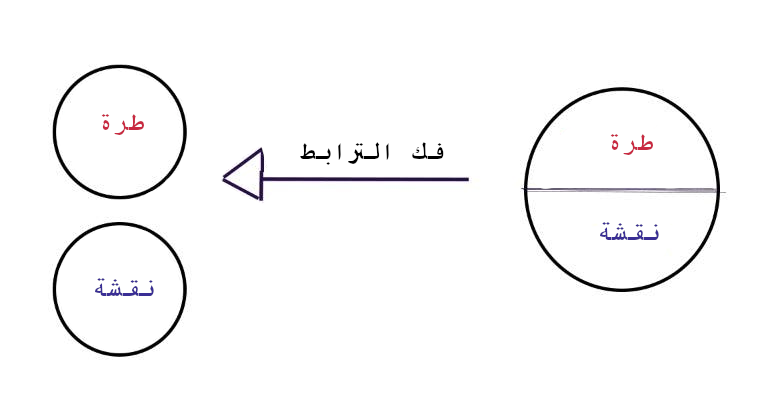
\includegraphics[width=\textwidth, height=5cm]{decoherence.png}
	\caption{مثال فك الترابط}
	\label{fig:dec}
\end{figure} \newpage


\section{الانتروبيا وانهيار الدالة الموجية}

قبل ما أن نتعلم عن انهيار الدالة الموجية, علينا ان نعرف ما هو
\textbf{الانتروبيا\dash \LR{Entropy}}.

\subsection{الانتروبيا}

الانتروبيا في نظرية المعلومات تعني المستوي المتوسط لالمعلومات أو المفاجأة المتأصلة في النتائج المحتملة للمتغير.

ويمكننا تعبيرها رياضيا بأستعمال قانون شانون الموضح كالتالي:

$$
{\displaystyle \mathrm{H}(X) := -\sum _{x\in {\mathcal {X}}}p(x)\log p(x)= \mathbb{E} [-\log p(X)],}
$$

حيث
$ \sum $
يرمز على مجموع القيم المحتملة لمتغير ما.
يختلف اختيار قاعدة اللوغاريتم باختلاف التطبيقات. تعطي القاعدة 2 وحدة البتات 
\emph{( أو "shannons" )} ، بينما تعطي القاعدة $ e $ "الوحدات الطبيعية" \emph{nat} ، وتعطي القاعدة 10 وحدات \emph{"dits"} أو \emph{"bans"} أو \emph{"hartleys"}.

\subsection{انهيار الدالة الموجية}

يحدث انهيار دالة الموجة عندما تقل الدالة الموجية - في البداية في تراكب عدة حالات - إلى حالة واحدة بسبب التفاعل مع العالم الخارجي. وهي تعتبر من خوارزميات الكم. لها استعمالات في علم الحاسب ايضا.

\begin{center}
	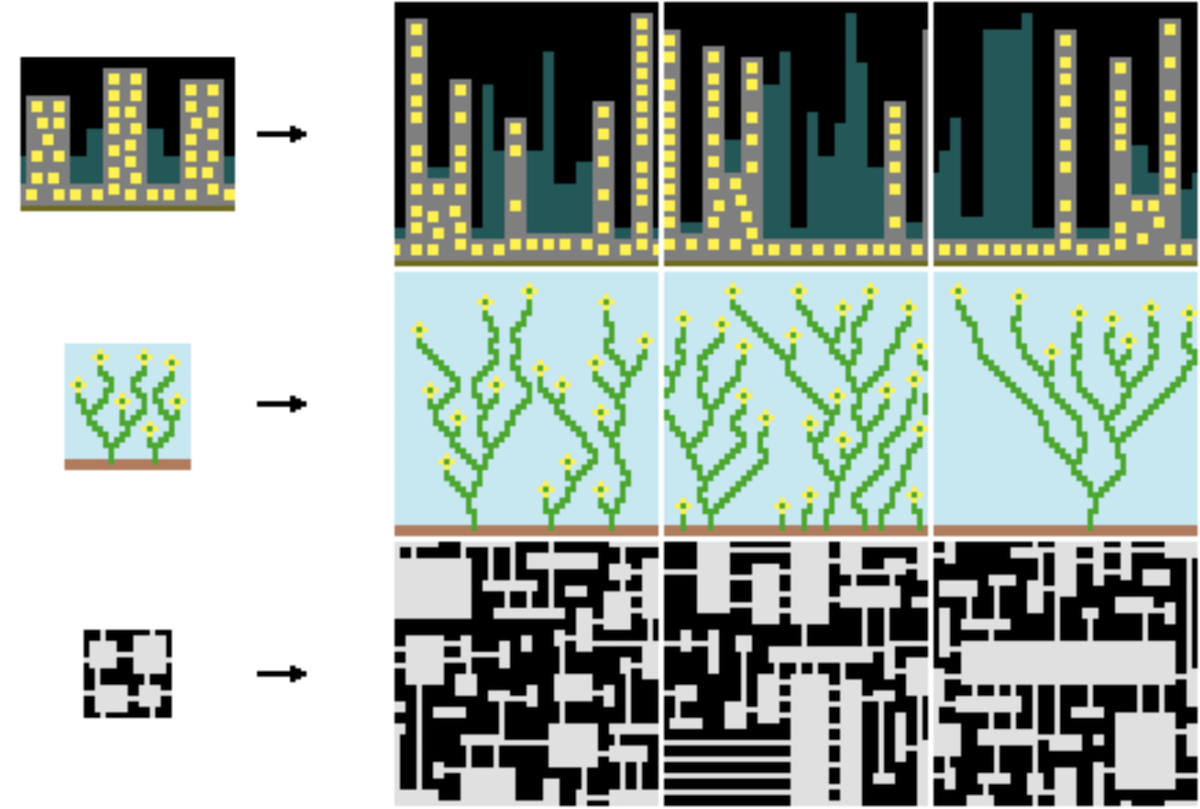
\includegraphics[width=\textwidth, height=7cm]{wfc-examples.png}
	\captionof{figure}{انهيار الدالة الموجية}
	\label{fig:wfc}
\end{center} \newpage

كما نرى في 
\textbf{الشكل \ref{fig:wfc}} 
ان نستطيع إنشاء صور كبرى من الصغرى بأستعمال انهيار الدالة الموجية, وهاكذا
تقوم انهيار الدالة الموجية بتعليم جهاز الكمبيوتر الخاص بك كيفية التكرار. تأخذ مدخلات نموذجية ، وتنتج مخرجات متولدة إجرائياً تبدو مثلها.

يتم استخدامه بشكل شائع لإنشاء الصور ، ولكنه قادر أيضًا على بناء المدن وحدائق التزلج والشعر.

\newpage

\chapter{الخاتمة}

\begin{center}
	
	وفي ختام بحثنا هذا نأمل ان أوضحنا ولخصنا المعلومات المفيدة وقد تلعمنا وحصلنا عن معرفة في فيزياء الكم, وعلم الحاسب, وما بذلك في العلوم. وانشاء الله كانت قرائتك  لهذا البحث ممتع.

\end{center}

\vspace*{0.3in}
\section{المراجع}

\selectlanguage{english}
\vspace*{0.5in}
\begin{itemize}
		\scriptsize
	\item \verb|https://en.wikipedia.org/wiki/Wave_function_collapse|
	\item \verb|https://en.wikipedia.org/wiki/Quantum_computing|
	\item \verb|https://en.wikipedia.org/wiki/Quantum_mechanics|
	\item \verb|https://en.wikipedia.org/wiki/Quantum_state#Pure_states|
	\item \verb|https://hackernoon.com/decoherence-quantum-computers-greatest-obstacle-67c74ae962b6|
	\item \verb|https://robertheaton.com/2018/12/17/wavefunction-collapse-algorithm/|
	\item \verb|https://www.techopedia.com/definition/34024/quantum-decoherence|
\end{itemize}

\selectlanguage{arabic}

\vspace*{0.2in}

\small
وتستطيع وجود كود\hspace{1pt}
\LaTeX \hspace{1pt}
 لهذا البحث في GitHub الرابط التالي:

 \begin{center}
	 \normalsize
	 \vspace*{0.3in}
 https://github.com/Chikmyvoltage/research\_project.git
 \end{center}

\vspace*{0.7in}

\begin{center}
	\LARGE
	والسلام عليكم ورحمة الله وبركاته
\end{center}
\end{document}

